\documentclass{standalone}
\usepackage{ tikz }
\usepackage{ xparse }
\usepackage{../../macros}

\begin{document}
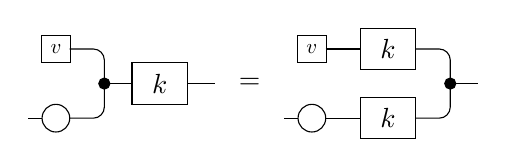
\begin{tikzpicture}[yscale=-1,x=1em,y=1.25em]

    \node [draw, minimum width=1em, minimum height=1em] at (0,0) {\scalebox{0.75}{$\mf{v}$}};

    \draw (-1,2) -- (-0.5,2);
    \draw (0,2) circle (0.5em);

    \draw [rounded corners] (0.5,2) -- (1.75,2) -- (1.75,1);
    \draw [rounded corners] (0.5,0) -- (1.75,0) -- (1.75,1);
    \filldraw (1.75,1) circle (2pt);
    \draw (1.75,1) -- (2.75,1);
    \node [draw, minimum width=2em, minimum height=1.5em] at (3.75,1) {$k$};
    \draw (4.75,1) -- (5.75,1);

    \node at (7,1) {$=$};

    \node [draw, minimum width=1em, minimum height=1em] at (9.25,0) {\scalebox{0.75}{$\mf{v}$}};
    \draw (9.75,0) -- (11,0);
    \node [draw, minimum width=2em, minimum height=1.5em] at (12,0) {$k$};
    \draw [rounded corners] (13,0) -- (14.25,0) -- (14.25,1);

    \draw (8.25,2) -- (8.75,2);
    \draw (9.25,2) circle (0.5em);
    \draw (9.75,2) -- (11,2);
    \node [draw, minimum width=2em, minimum height=1.5em] at (12,2) {$k$};
    \draw [rounded corners] (13,2) -- (14.25,2) -- (14.25,1);
    \filldraw (14.25,1) circle (2pt);
    \draw (14.25,1) -- (15.25,1);

\end{tikzpicture}
\end{document}